\subsection{Caso Particular GeM}
\label{subsec:exp8}
\begin{LaTeXdescription}
    \item[Objetivo] Analizar cuan ``justo'' es GeM, para un caso particular en
        el cual no haya dudas sobre lo que es justo y lo que no\footnote{O que
        haya muy poca probabilidad de que haya dudas al respecto.}.\\

    \item[Proposici\'on] Nos interesa analizar cu\'an ''justo'' es GeM para
        cierta definici\'on de justicia. Consideremos el caso de un torneo en
        que el equipo A le gana a todos los equipos salvo a B, y B pierde todos
        los partidos salvo el que le gana a A. Bajo nuestra definición de
        ''justicia'' o ''equidad'', o un aspecto de ella, A deber\'ia estar
        seguro por encima de B y B no deber\'ia estar por encima de muchos
        equipos (ya que perdi\'o contra todos). Observamos que en el caso del
        f\'utbol y su ránking 3-1-0 (o el esquema antiguo, 2-1-0) efectivamente
        B estar\'ia en la \'ultima posici\'on y A estar\'ia en la primera
        (eventualmente compartiendo dichas posiciones con alg\'un otro equipo).
        Entendemos entonces que este caso particular el ranking 3-1-0 es
        ''justo'' en este aspecto. Pero intu\'imos que esto no ser\'a lo que
        ocurra con GeM, ya que en el grafo de la instancia, A tiene un \'unico
        eje saliente (hacia B) y 18 entrantes, con lo cual su arista deber\'ia
        hacer subir mucho a B en el ranking.\\

    \item[Hip\'otesis] PageRank/GeM no es ''justo'' en cuanto al aspecto
        mencionado.\\

    \item[M\'etodo de Experimentaci\'on] Generamos una instancia de 20 equipos
        todos contra todos, donde existen A y B como se describieron. Entre los
        dem\'as equipos hacemos que el ganador sea aleatorios (con semilla =
        5). Todos los partidos terminan 1 a 0. Ejecutamos GeM y observamos el
        ranking final para diferentes valores de $\alpha$ (el factor de
        navegaci\'on).

    \item[Resultados, an\'alisis y discusi\'on] Lo primero que observamos es que B no ascendió al primer lugar para ningún valor de $\alpha$, lo cual era esperable dados los resultados del experimento 7 pero no deja de darnos cierta ``tranquilidad''. Sin embargo, y como se puede ver en la figura \ref{fig:exp8_posB}, la posición del equipo B sí mejora significativamente ya para valores pequeños de $\alpha$: ya un valor de $\alpha = 0.1$ deja a B 6to en el ránking, y a partir de $\alpha = 0.4$ pasa a estar 2do. Consideramos entonces que se confirmó nuestra hipótesis en el sentido de que GeM no es ``justo'' en un caso del estilo. Como ya postulamos en el experimento 7, no parece ``justo'' que un equipo prácticamente invicto que tuvo un ``mal día'' le permita a otro equipo salir 2do en una competencia en la que perdió con cuanto rival se cruzó.
    
    Podemos concluir entonces que los valores más ``justos'' de $\alpha$ serían los más bajos, dado que le dan menos importancia a estas situaciones extrañas pero perfectamente posibles en cualquier deporte.
    
\end{LaTeXdescription}

\begin{wrapfigure}{l}{0.5\textwidth}
    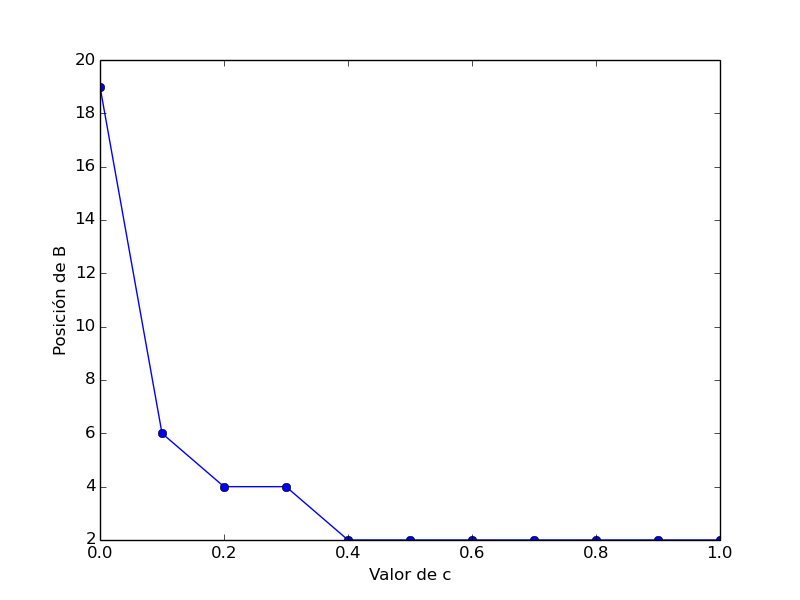
\includegraphics[width=0.5\textwidth]{exp8_posicion_B.png}
    \caption{Posici\'on del equipo B en el ranking en funci\'on del factor
        $\alpha$ ($c=\alpha$)}
    \label{fig:exp8_posB}
\end{wrapfigure}
\noindent
